\documentclass[10pt,conference]{IEEEtran}

\usepackage[]{hyperref}
\usepackage[]{graphicx}
\usepackage[]{authblk}
\usepackage{multirow}
\usepackage{multicol}

\begin{document}
\title{Miniproject 1 Report}
\author[1]{Olivier Cloux}
\affil[1]{Department of Computer Science, EPFL}

\maketitle

\begin{abstract}
Some content
\end{abstract}

\section{Introduction}
Deep Learners have been around for quite some time now \cite{noauthor_deep_2020}. But only recently have we started to unlock their potential, thanks to faster than ever hardware. Among some properties of Deep Neural Networks (DNN), we can cite the use of auxiliary loss, and the use of weight sharing.

Behind the idea of weight sharing is the supposition that similar parts of the input can affect the output similarly. There are multiple ways to implement this, either by using a Siamese Networks \cite{noauthor_siamese_2020}, or by using so-called Convolutional Neural Networks \cite{noauthor_convolutional_2020}. This is notably useful for images-like data, where we can suppose some features detection (colors, angles, edges,\ldots) may be useful at multiple parts of the input.

The second interesting property, auxiliary loss, was introduced by a GoogLeNet paper \cite{szegedy_going_2014}, and is roughly defined as using additional properties as the target. Totally unrelated example, if we want to predict which of two hand-written digits is greater than the other, we could try and predict the actual digits to train our network, and use this help to update our network for the former task.

\section{Task}
In this experiment, we will try and predict which of two hand-written digits is greater than the other\footnote{I lied earlier, it wasn't unrelated}. The data we use is a slight modification of the MNIST \cite{lecun_mnist_1998}, where each entry is composed of two ordered but unsorted handwritten digits. The label to predict is a binary value, indicating which of both is the greatest. Note we also have at hand the original labels (indicating the actual value of each digit), but only use it in certain cases.

Each image is a $14\times14$ grayscale image. So each item is a $2\times14\times14$ tensor.


\section{Models and methods}
As we wish to investigate the effect of weight sharing and auxiliary loss, it makes sense to create 4 models, combining these criterions.
\begin{table}[h]
    \begin{tabular}{l|c|c}
        & No auxiliary loss & Auxiliary loss\\
        \hline
        No weight sharing & Baseline & Baseline + Auxiliary\\
        \hline
        Weight sharing & CNN & CNN + Auxiliary
    \end{tabular}
    \label{tab:names_models}
    \caption{Names of models considered}
\end{table}
As you can see, we really only have two models (\textit{Baseline} and \textit{CNN}). Both of them always output a binary classification (our main goal), and a 10-classification (the digits of the numbers). But if we don't wish to use them, we simply discard the latter.

Furthermore, we also use l2-regularization to help overfitting and reduce the amplitude of the weights.

\subsection{Model 'Baseline'}
This first simple model is composed of 4 layers, all quite similar to each other. You can see the structure in Table \ref{tab:structure_baseline}. The first three layers serve to create the classification 10 (the value of each digit). Then this layer continues and is reduced to a size 2, the binary value of which is greater.
\begin{table}
    \begin{tabular}{c|c||c}
        Layer & Name & Output (if applicable)\\
        \hline\hline
        \multirow{4}{*}{1} & Fully Connected 196$|$392 $\to$ 200\\
        & Batch Normalization\\
        & ReLU\\
        & MaxPool 1d (Kernel size 2, stride 2)\\
        \hline
        \multicolumn{1}{c}{} & Dropout 50\% & \\
        \hline
        \multirow{4}{*}{2} & Fully Connected 100 $\to$ 256\\
        & Batch Normalization\\
        & ReLU\\
        & MaxPool 1d (Kernel size 2)\\
        \hline
        \multicolumn{1}{c}{} & Dropout 50\% & \\
        \hline
        3 & Fully Connected 128 $\to$ 10 & Output classification 10\\
        \hline
        \multirow{2}{*}{4} & Fully Connected 20 $\to$ 2\\
        & ReLU & Output classification 2
    \end{tabular}
    \caption{Structure of the Baseline network}
    \label{tab:structure_baseline}
\end{table}
Note than between layers 1 and 2, and between layers 2 and 3 we apply a dropout of 50\% to reduce overfitting. Also, as mentioned earlier, the output 10-classification is only used if we wish to use auxiliary loss. Finally, note that the input is either 196 or 392. The first case corresponds to an input of $14 \times 14$ and is used when we use auxiliary loss. In this case, we need to split images and identify them accordingly. One input is then 196 pixels. The latter is twice that amount, and is used without auxiliary loss, when an input is 2 images (hence $2\cdot 196$).

\subsection{Model 'CNN'}
This network is relatively similar, with the replacement of some Fully Connected layers by 2D Convolutional layers. You can see the details in table

\begin{table}
    \begin{tabular}{c|c||c}
        Layer & Name & Output (if applicable)\\
        \hline\hline
        \multirow{4}{*}{1} & Conv. $1|2 \to 16$, kern. 5, padding 3\\
        & Batch Normalization\\
        & ReLU\\
        & MaxPool (Kernel size 2)\\
        \hline
        \multirow{4}{*}{2} & Conv. $16 \to 20$. kern. 5, padding 3\\
        & Batch Normalization\\
        & ReLU\\
        & MaxPool (Kernel size 2)\\
        \hline
        \multirow{2}{*}{3} & Fully Connected $500 \to 300$\\
        & ReLU\\
        \hline
        4 & Fully Connected $300 \to 10$ & Output classification 10\\
        \hline
        \multirow{2}{*}{5} & Fully Connected $10 \to 2$\\
        & ReLU & Output classification 2
    \end{tabular}
    \caption{Structure of the CNN networks}
    \label{tab:struct_cnn}
\end{table}

\subsection{Method}
In order to compare the models between them, we created a testing pipeline, through which they are all passed. The same actions are repeated for a certain amount of \textit{rounds} (about 20) to obtain averaged results. At each round, a thousand training and testing items are created. If we wish to use auxiliary loss, the data is flattened. Then the network is trained (logging the loss), and finally we compute the training and testing error. All those steps are timed. Results of each rounds are returned for analysis.

The training is quite straightforward. During a count of epochs, we again repeat loop, splitting the data in batches, account for the 2-classification, drop or keep the 10-classification, and add $\ell_2$ regularization. Finally we apply the backward pass and reset the gradients.

The optimization was made using the Adam optimizer, on CrossEntropy loss. The total loss is either simply the ``normal'' loss, or the sum of it with the Auxiliary loss.
\subsection{Parameters}
The following parameters were used:
\begin{multicols}{2}
    \begin{itemize}
        \item 20 rounds
        \item 25 epochs
        \item Mini-batch size 100
        \item Cross-Entropy loss
        \item Adam Optimizer
        \item lr Baselines $1e-3$
        \item lr CNNs $5e-4$
        \item $\ell_2$ 0.1
    \end{itemize}
\end{multicols}
\section{Results}
\subsection{Training loss}
For each model, we logged the loss while training. This allows us to see how fast a network will converge. Loss is averaged across rounds, and we plot the deviation of each step. You can see the results at Figure \ref{fig:training_losses}.
\begin{figure}
    \centering
    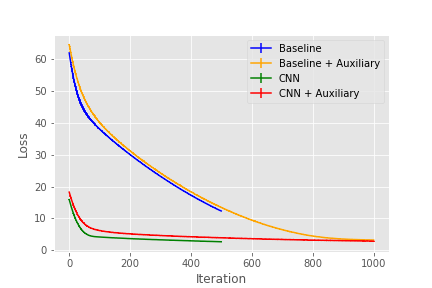
\includegraphics[scale=0.6]{../images/rounds_losses}
    \caption{Evolution of the training losses}
    \label{fig:training_losses}
\end{figure}
This shows the CNN models tend to have a better training loss, and reach their limit quite fast, while Baseline models can start far worse, and take some time to reach equivalent performances. Note that this could be further tweaked with cross-validation and hyperparameters optimization, but this is out of the scope of this project, for which we used ``good enough'' hyperparameters.

\subsection{Errors and Time}
The above only shows us the evolution of the training loss. We now look at three interesting measures: training error, testing error, and training time. Figure \ref{fig:err_time_rounds} shows these results
\begin{figure}
    \centering
    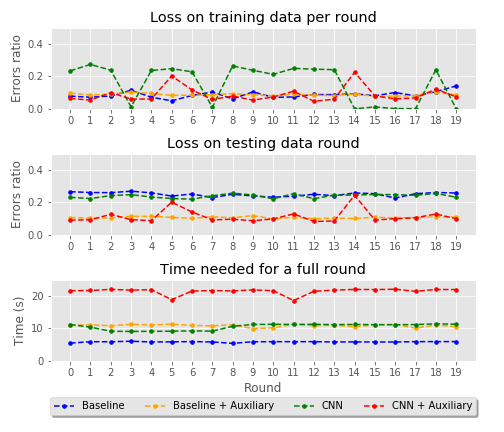
\includegraphics[scale=0.49]{../images/comparison.png}
    \caption{Errors and Times across rounds}
    \label{fig:err_time_rounds}
\end{figure}
There are some conclusions that arise. First of all, using the auxiliary loss yields much better results on the testing set (actually the most important one). Also, the more complex a model is, the longer the training takes (no surprise there). Interestingly, all models have a similar training error, except for CNN, that oscillates between two very distinct states. You can find a summary of the mean/std for these metrics in Table \ref{tab:recap}.
\begin{table}
    \begin{tabular}{l||ccc}
        & Train error [\%] & Test error [\%] & Time/round [s]\\
        Baseline & $8.7 \pm 2.0$ & $25.0 \pm 1.2 $ & $5.8 \pm 0.15$ \\
        \hline
        Baseline + Aux & $8.8 \pm 0.7$ & $10.6 \pm 0.5$ & $10.8 \pm 0.4$ \\
        \hline
        CNN & $15.9 \pm 11.6$ & $23.9 \pm 1.19$ & $10.5 \pm 0.9$ \\
        \hline
        CNN + Aux & $8.8 \pm 4.8$ & $11.3 \pm 4.1$ & $21.4 \pm 0.9$
    \end{tabular}
    \caption{Recap of Train/Test error and round times}
    \label{tab:recap}
\end{table}
Using the above results, there we can draw some conclusions.
\begin{itemize}
    \item CNN is more complex (and thus longer to train) than Baseline.
    \item Using auxiliary loss makes the training longer even, regardless of the underlying network.
    \item Baseline takes more epochs, but can achieve comparable results.
\end{itemize}
\section{Summary}
To summarize the above, the lessons to take home are that:
\begin{itemize}
    \item If you lack data, use weight sharing, it will allow for a much faster convergence, even if each epoch is significantly slower.
    \item With more data, the weight sharing may not be necessary, but can probably achieve better results with some additional tweaks (notably of hyperparameters).
    \item Use all the data at your disposal. There is no point in discarding some of it. Even if it's not the main label we are trying to classify, it's still better to use it for auxiliary loss.
\end{itemize}
There is still work left to obtain a more precise idea. First of all, we could compare more networks, with less differences between them. Also, we could compare more architectures of weight sharing, other than CNN. Siamese nets, mentioned earlier, could be an interesting track. Finally, some more work could be done on hyperparameters to obtain ``the best'' of each network, to have a more sensible comparison.
\bibliographystyle{IEEEtran}
\bibliography{dl_report}

\end{document}
